% !TeX root = ../proceedings.tex

\section{Design Challenges}
\subsection{How should the user access the application?}
A menu screen is an essential part of any application. The menu is something every user has experience with and it is the first thing a user is met with when running an application. This means that the menu has to consist of certain classic elements.\par A user needs a way to close the application. On mobile phones nowadays this can be done with 'return' buttons on the phone, but applications generally have a built in exit function.\par
The user also needs to have some sort of options menu and guidelines. This is a must for this application. Stacking LEGO seems simple and intuitive, but all the operations and possibilities is something that can confuse a potential user. \par
Lastly the menu needs to have an easy access to the LEGO session itself. It shouldn't be complicated for the user to start a new LEGO session. 
\subsection{The Main Menu}
\begin{figure}[h]
	\centering
	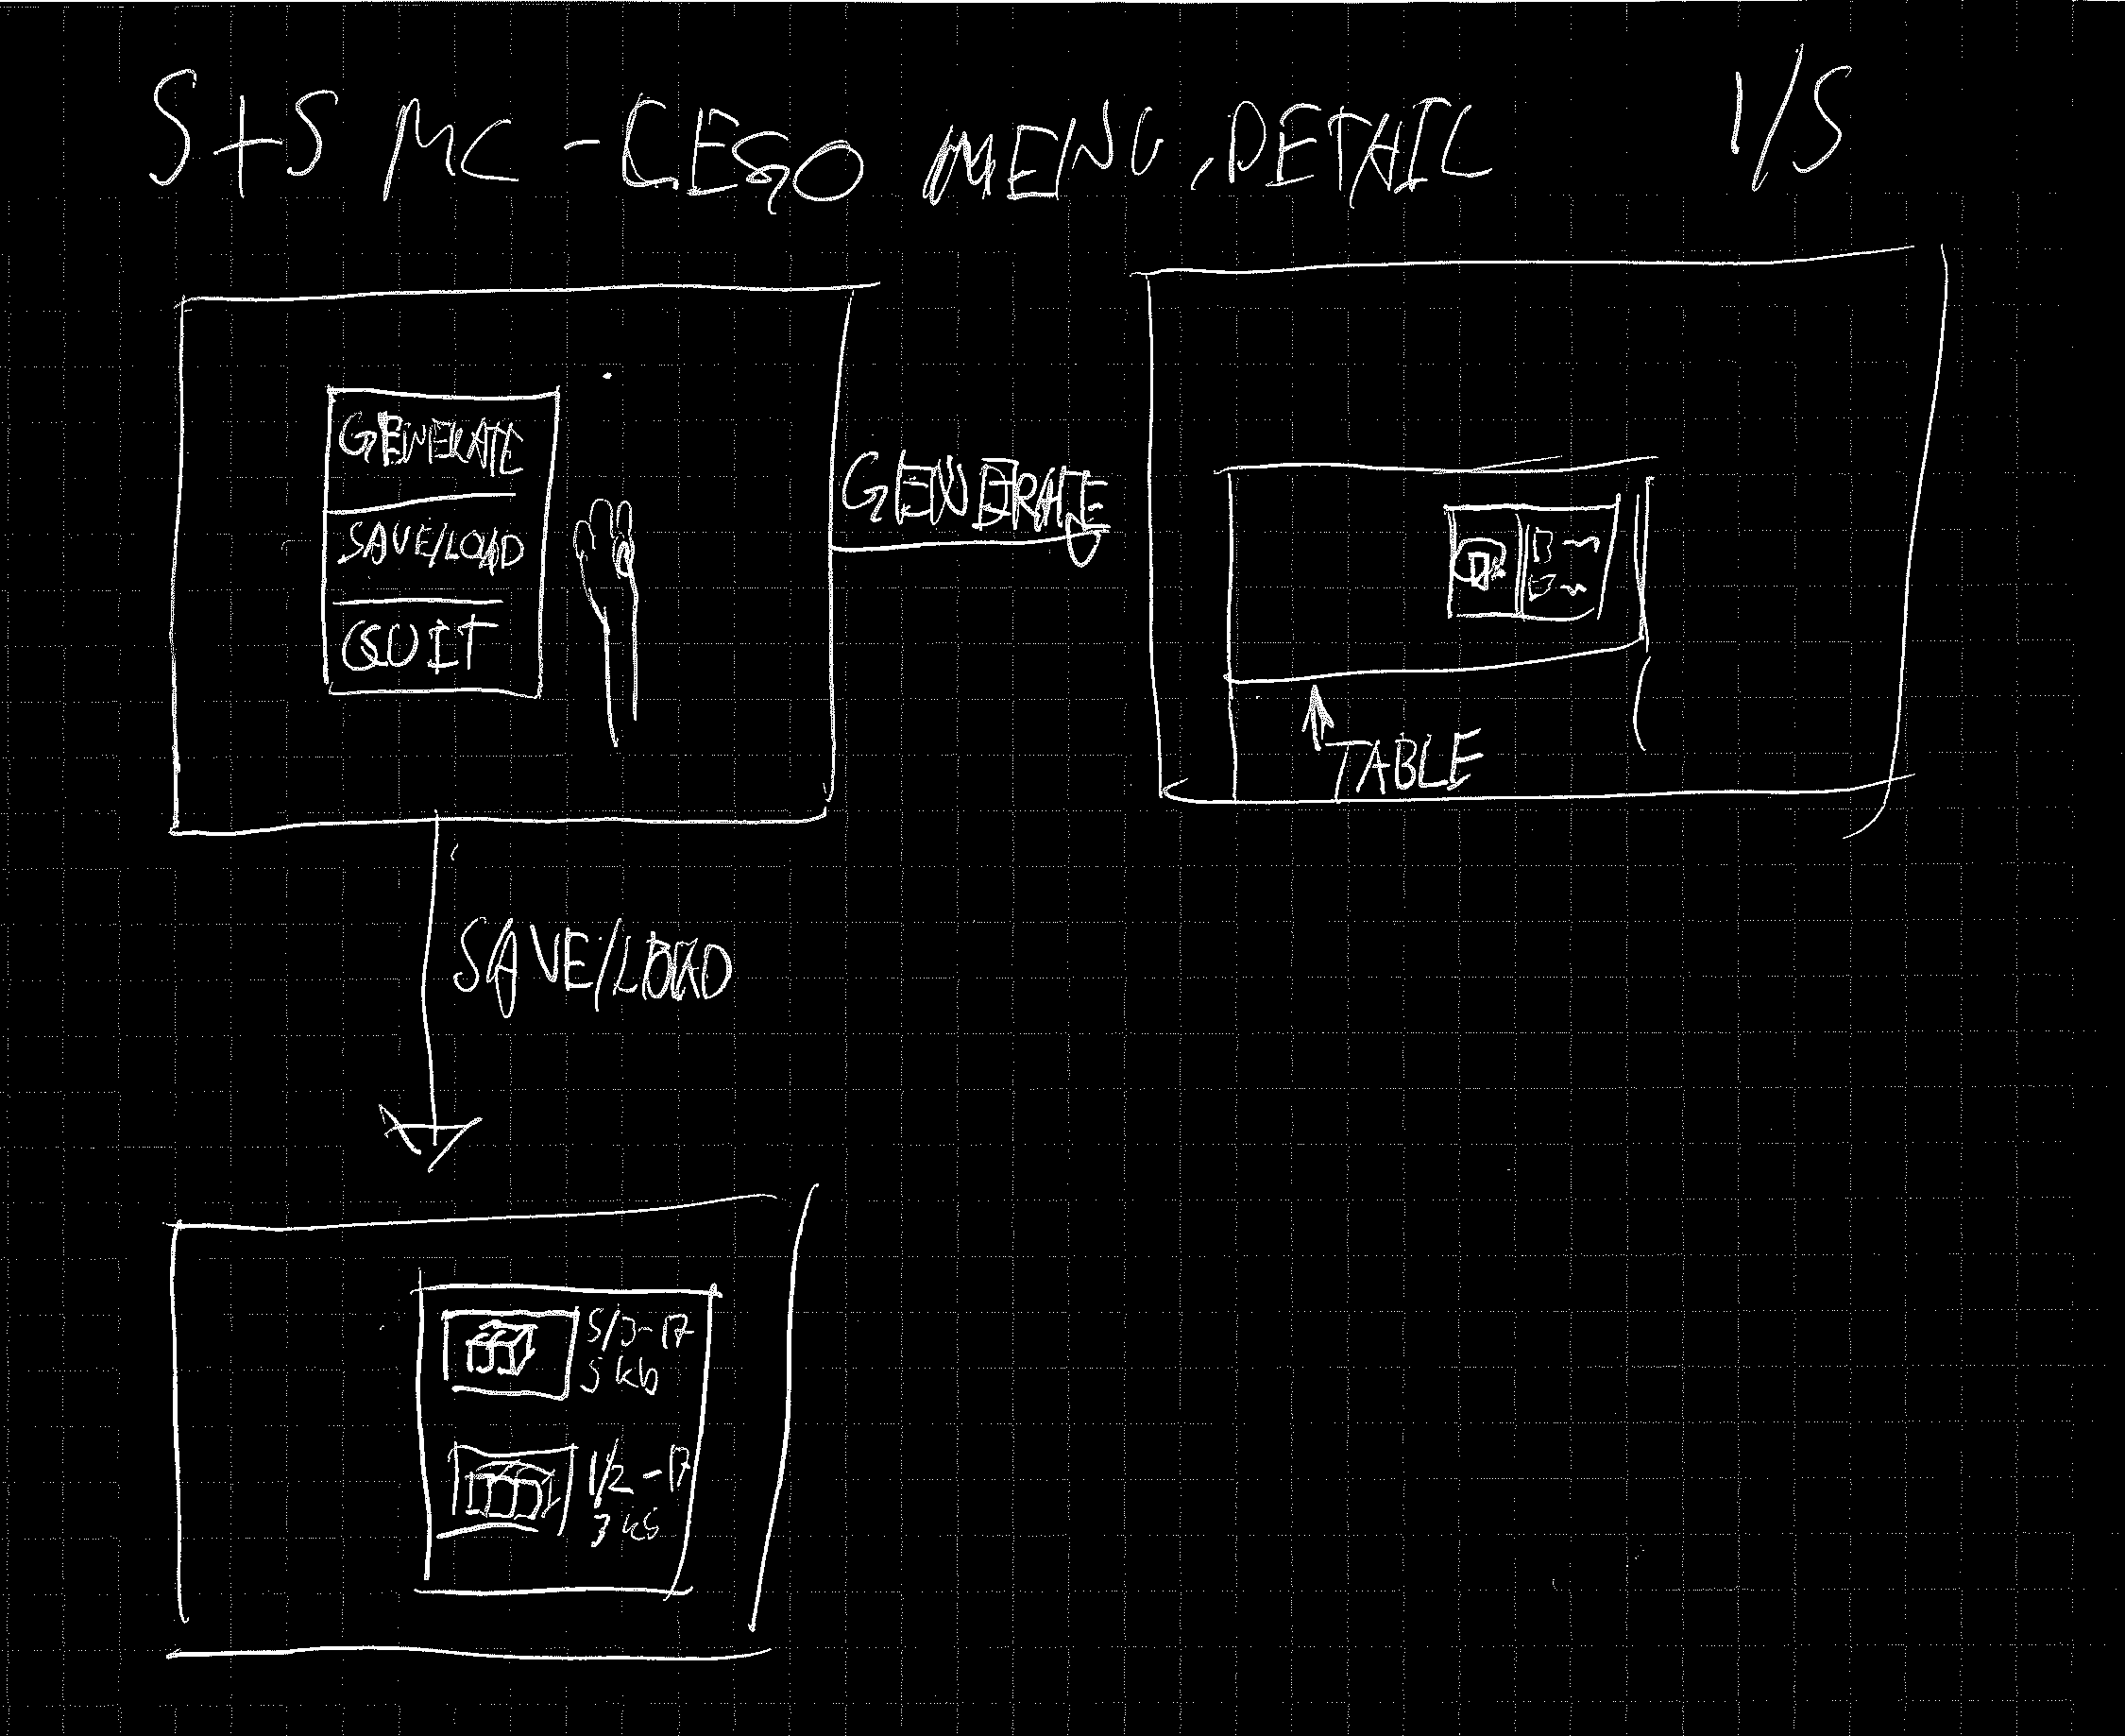
\includegraphics[width=0.7\linewidth]{figures/Menu/menu8}
	\caption{The first idea of a seperate Main Menu screen}
	\label{fig:menu8}
\end{figure}
We initially though about having a main menu screen. Just as figure\ref{fig:menu8} illustrates. The user would open the Hololens application, and be met with a menu screen, where actions such as generating a play area, loading and saving a game and a way to quit the application. \par
The sketches were generated following a '5 plus 5' approach. Each member of the group drew 5 different ideas of a main menu screen. One common theme in the sketching of the main menu was separation of the design of the menu and the interaction with the menu, and the difficulties with making that separation.\par
\begin{figure}[h]
	\centering
	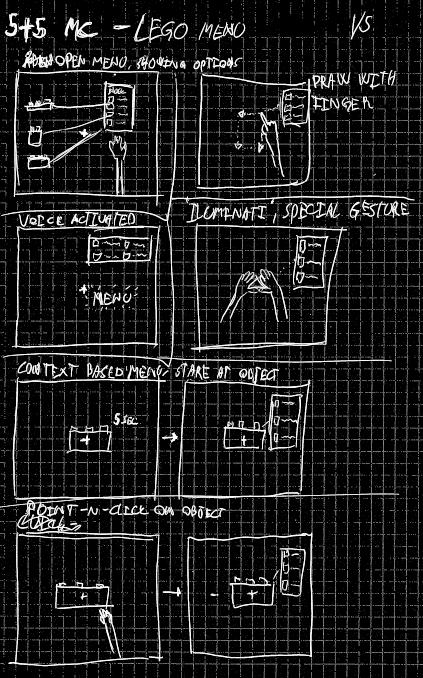
\includegraphics[width=0.7\linewidth]{figures/Menu/menu5}
	\caption{A focus on gestures rather than design, impacted the design. The figure shows 5 different ways of creating an interactive menu for the user to use.}
	\label{fig:menugesture}
\end{figure}
In quite a few of the earlier sketches, interaction with the menu was in focus rather then the design of the menu, just as figure \ref{fig:menugesture} depicts.\par
The possibilities with the HoloLens gestures and the augmented reality made it apparent that the menu had to be movable, either by closing and opening with the gestures available, or being able to move it around the play area. 

\subsection{The generator board}
After discussing menus in the context of the Hololens, it became apparent that there was a need for a menu that could be placed and interacted with in the real world. Using the spatial mapping and spatial understanding capabilities of the Hololens, different designs of the so called 'generator board' were done. Figure \ref{fig:genboard1} is a sketch of what functionalities the generator board should have.
\begin{figure}[h]
	\centering
	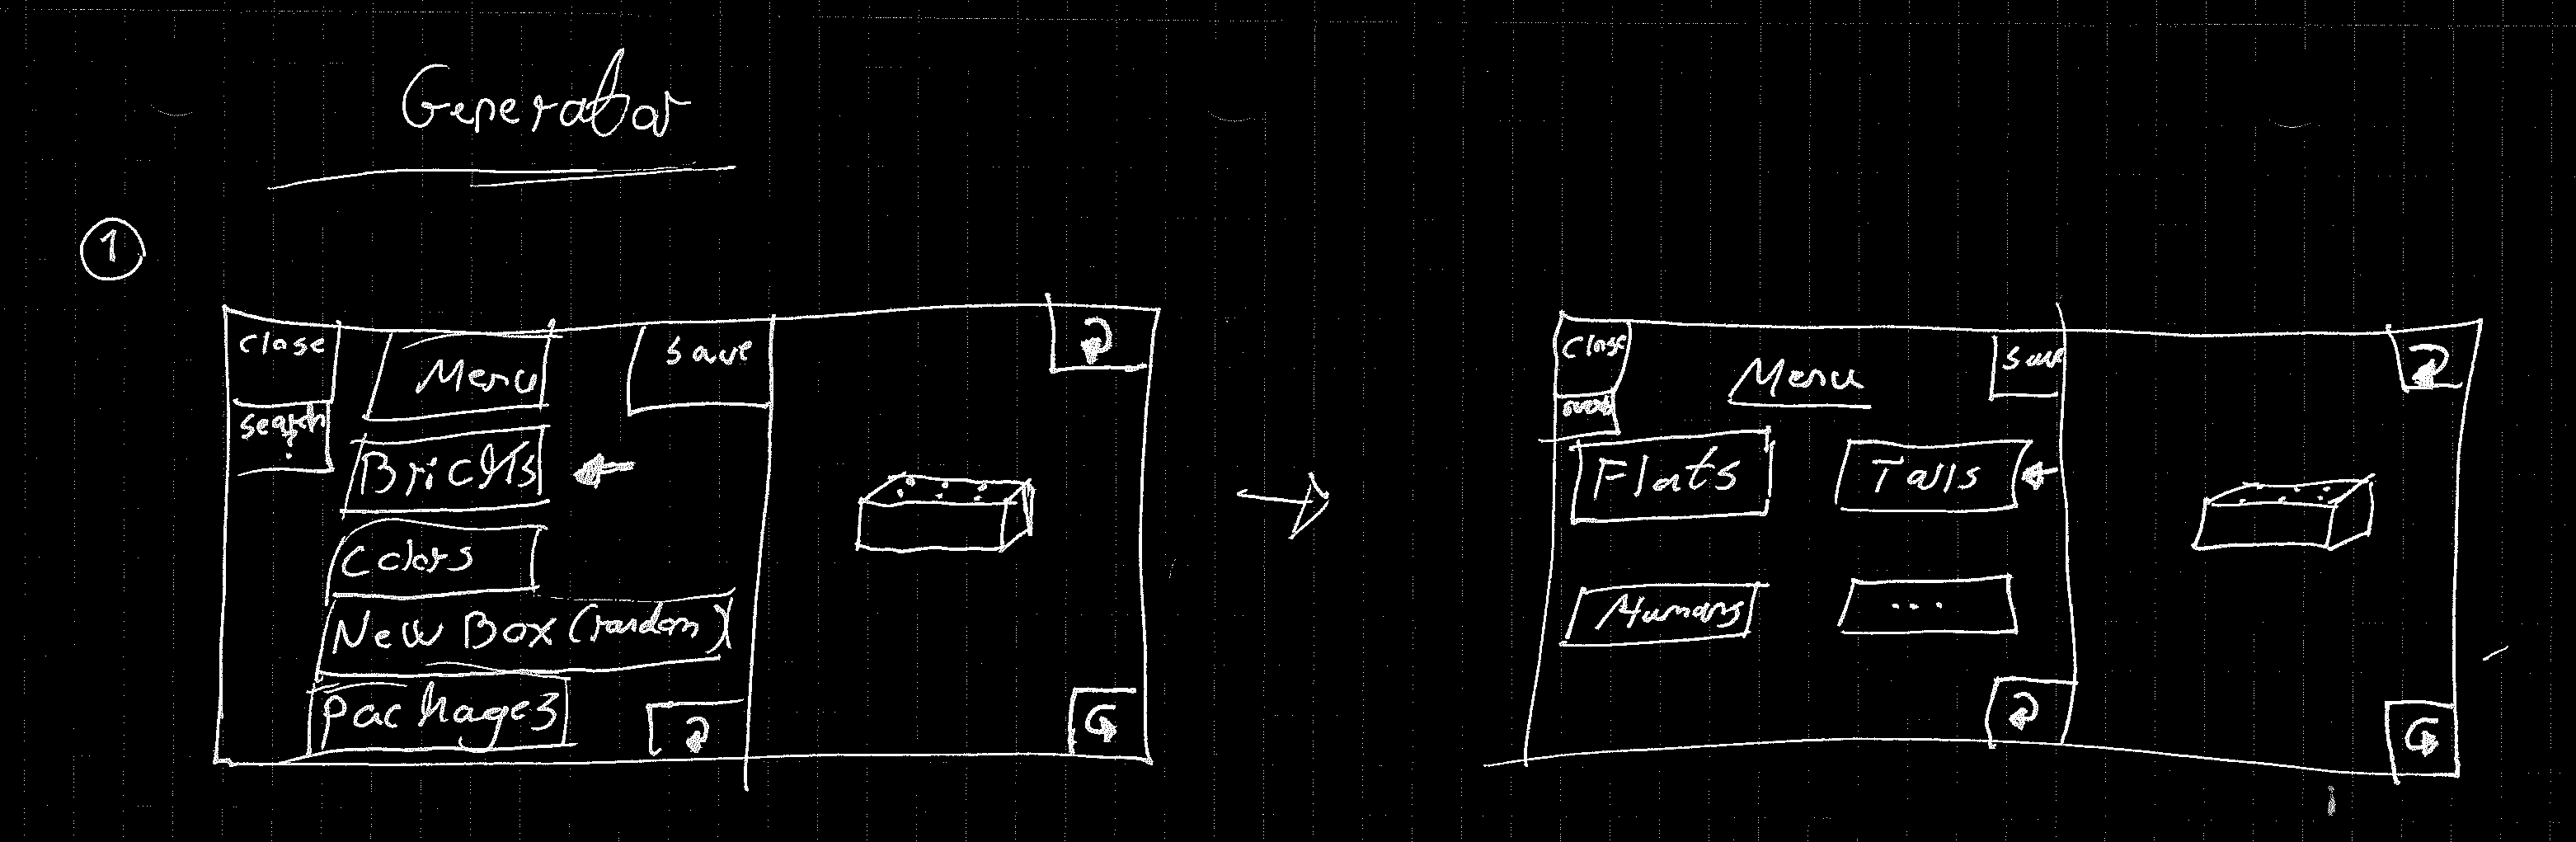
\includegraphics[width=0.7\columnwidth]{figures/Generator/gen5.png}
	\caption{An initial sketch of how the generator board could look like. The menu screen has alot of functionalities, and the actions chosen happen on the right side.}~\label{fig:genboard1}
\end{figure}
The main idea was to have a generator board that was accompanied with functionalites to alter the blocks, but also to be interactive and movable in the play area.\par
We designed the generator board as a tablet device, making it more natural for the user to interact with. It follows the idea of the sketch in figure \ref{fig:gentablet}, where the generator board is placed on the table.
\begin{figure}[h]
	\centering
	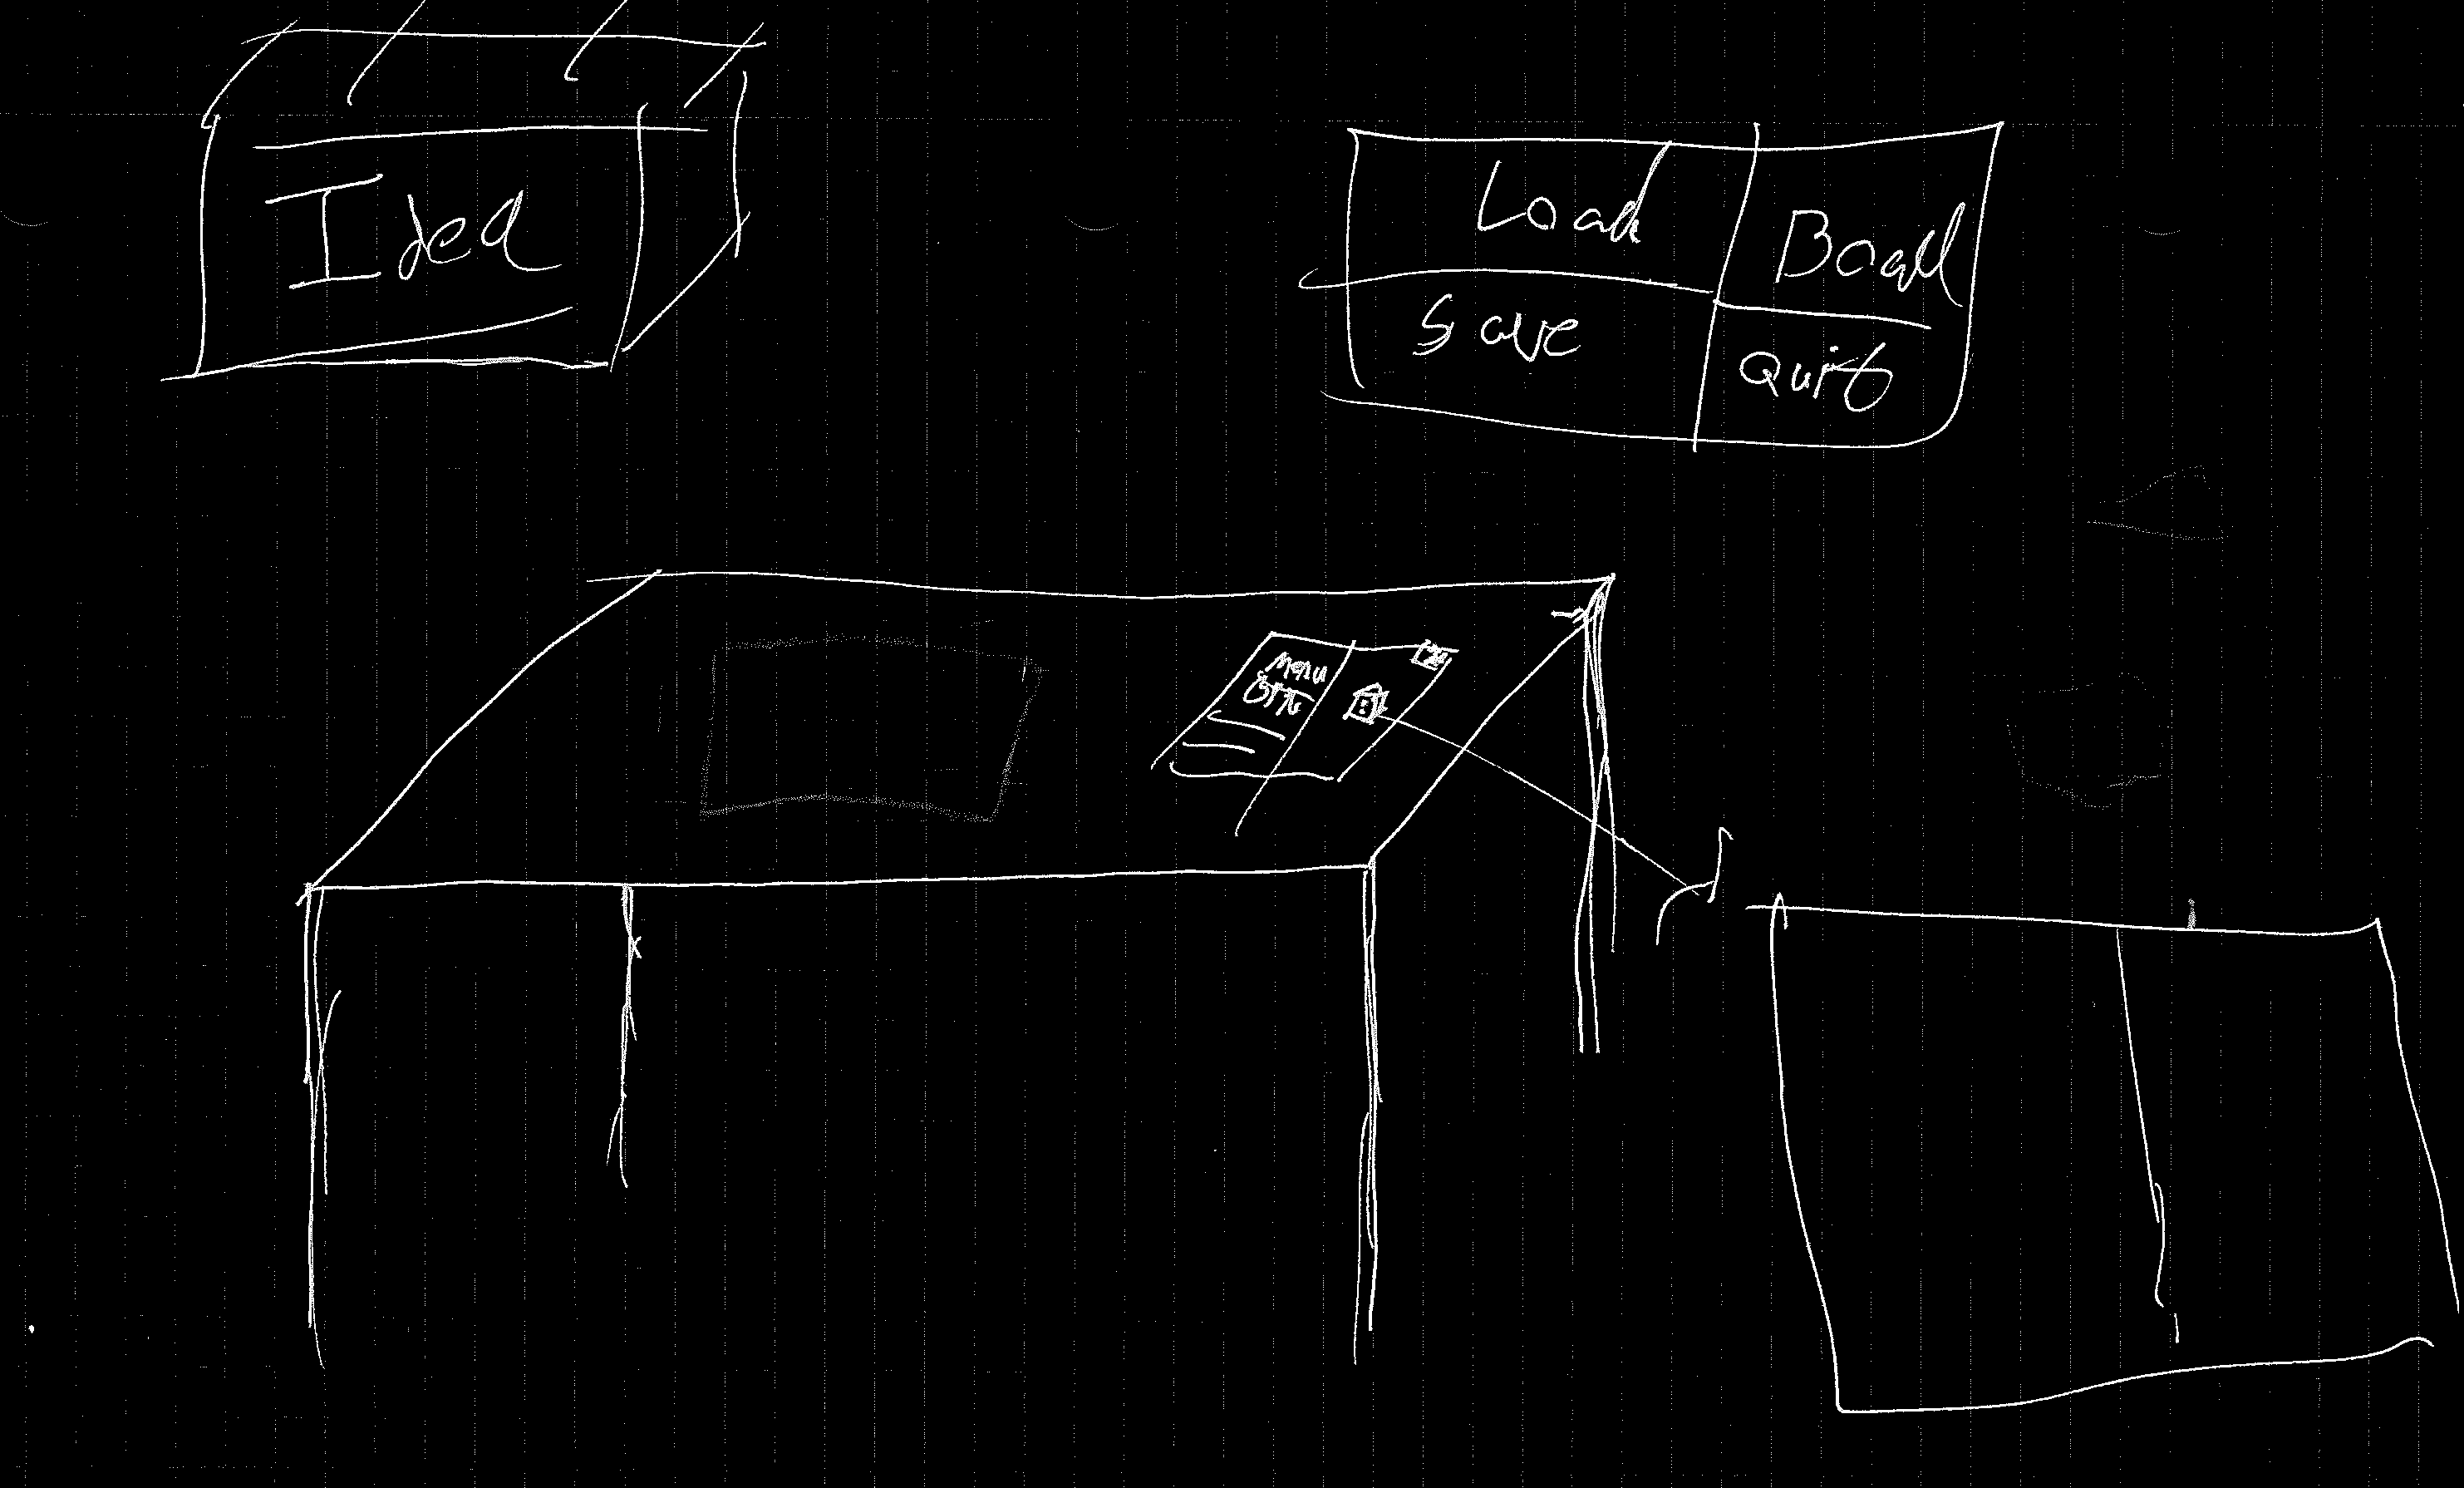
\includegraphics[width=0.7\columnwidth]{figures/Generator/gen6.png}
	\caption{First sketch of the generator board as a movable object. Here placed on the table, spawning blocks on the table.}~\label{fig:gentablet}
\end{figure}
 Being a solid object the user knows, makes it more intuitive and natural for the user to lift, move and place the menu on a surface like a table or the floor.
 \begin{figure}[h]
 	\centering
 	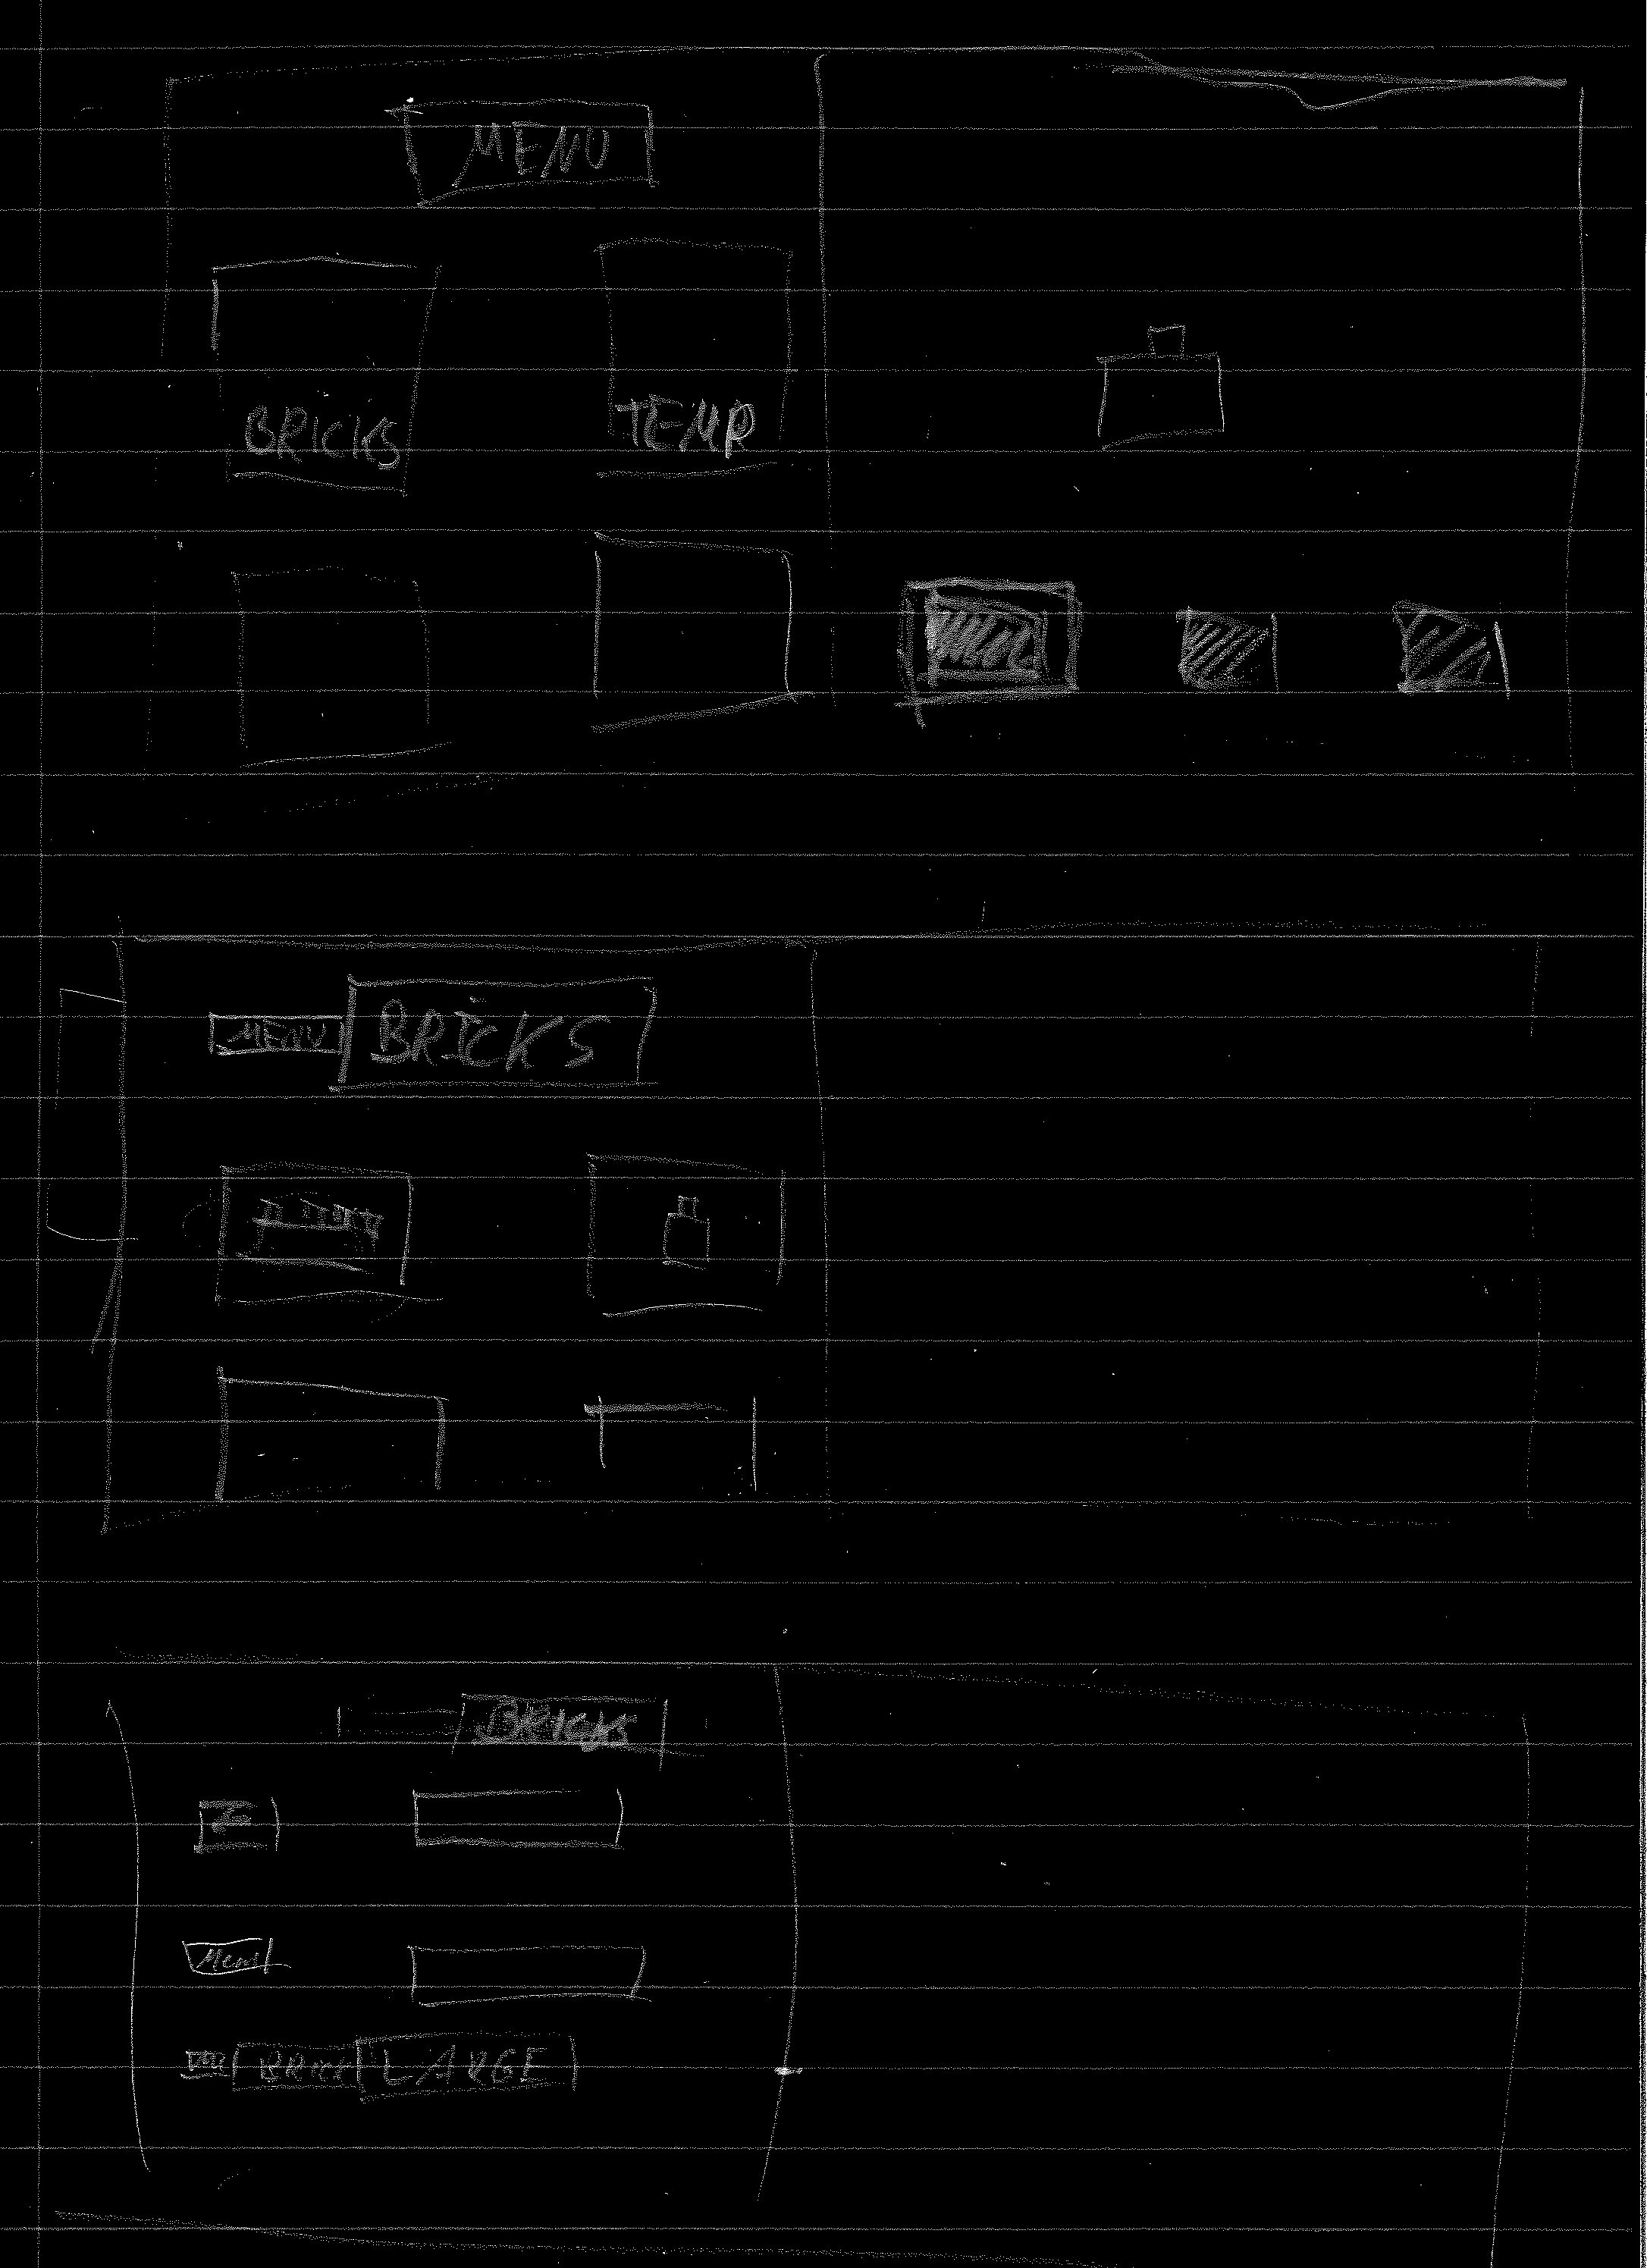
\includegraphics[width=0.7\columnwidth]{figures/Generator/gen4_22.png}
 	\caption{An initial sketch of the functionalities within the generator board. It has various buttons, such as generating a specific block, a template screen with predefined figures etc.}~\label{fig:genfuncs}
 \end{figure}
 Figure \ref{fig:genfuncs} show some of the thoughts made towards the functionality and buttons inside the generator board. Another concern was that each menu needed a 'back' button so the user could return to the main screen. Colors are also a must to be changed. 
\subsection{Design decisions}
\begin{figure}[h]
	\centering
	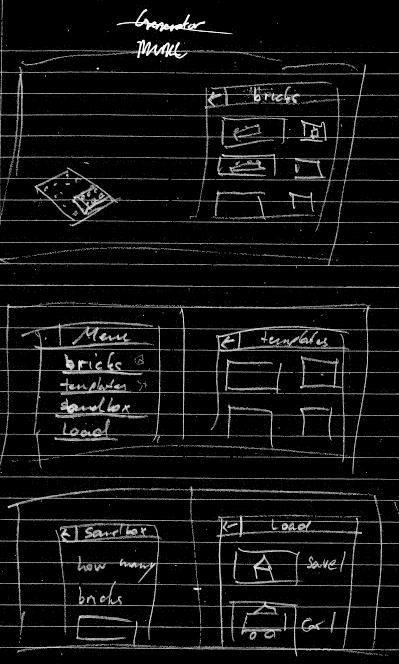
\includegraphics[width=0.5\columnwidth]{figures/Menu/menu1.png}
	\caption{Initial Main Menu screen with big button, simple interaction and short descriptions.}~\label{fig:genboard}
\end{figure}
During the sketching phase, several design choices were discussed. One of the very first decisions made was the overall look of the menu. The choice of big buttons, clear visual cues and short textual descriptions was present in almost all of the sketches in the early design phase, as seen in figure \ref{fig:genboard}. The generator board needed to have the same simple design. The main menu and the generator board should not be overcomplicated, but not sparse in functions either. 
\subsection{Moving away from a main menu}
As the development of the application progressed it became more and more apparent that an actual main menu was not necessary. All the interactions needed for the prototype could be implemented through the tablet looking generator board and could ease user interaction with the application. Instead of going through a main menu and then having the generator which contains the functionality for working with the LEGO bricks, spawning the generator board at the application start up and "cutting out the middleman" seemed as a natural choice for this prototype. Granted, with an eventual increase in functionality and complexity of the application, a root/main menu might prove useful as to not clutter the users experience when they are building as opposed to when they are in the main menu setting options, loading scenarios, downloading templates etc.